\documentclass[usenames,dvipsnames,aspectratio=169]{beamer}

\usebackgroundtemplate%
{%
    
\includegraphics[width=\paperwidth,height=\paperheight]{it_1.png}%
}
\beamertemplatenavigationsymbolsempty
\usepackage{pgfpages}
\setbeameroption{show notes}
\usepackage[portuguese]{babel}
\graphicspath{{./images/}{./figures/}}
\usepackage[utf8]{inputenc}
\usepackage{braket}
\usepackage{amsmath}
\usepackage{xcolor}
\title{Mini-workshop \LaTeX and Git}
\author{Daniel Pereira\\ Armando Nolasco Pinto}
\institute{Universidade de Aveiro}


% Color definition
\definecolor{title}{RGB}{68,85,95}
\definecolor{author}{RGB}{120,144,159}
\definecolor{mainTextColor}{RGB}{55,59,61}
\definecolor{mainEquationColor}{RGB}{0,0,0}
\color{mainTextColor}

% Itemize tick definition
\newcommand{\aitem}{\item[$\cdot$]}
\newcommand{\bitem}{\item[-]}
\newcommand{\citem}{\item[$\ast$]}

\setbeamercolor{frametitle}{fg=title}
\setbeamercolor{normal text}{fg=mainTextColor}

\AtBeginSection[]{
  \begin{frame}
  \vfill
  \centering
   \color{title} \sffamily \noindent \Huge
    \insertsectionhead\par%
  \vfill
  \end{frame}
}

\AtBeginSubsection[]{
  \begin{frame}
  \vfill
  \centering
   \color{title} \sffamily \noindent
%    \Huge \insertsectionhead\par%
    \Large\insertsubsectionhead\par%
  \vfill
  \end{frame}
}


% 30 LaTeX slides

\begin{document}

{
\usebackgroundtemplate{
\includegraphics[width=\paperwidth]{it_0.png}}%
\begin{frame}
\color{black} \sffamily \noindent \large
\hspace*{1cm}
\begin{minipage}{10cm}
\vspace*{.4cm}
\begin{flushleft}
 \color{title} \sffamily \noindent \Large
\textbf{Mini-workshop \LaTeX and Git}
\end{flushleft}
\end{minipage}
\vspace*{.8cm}\\
%
~\\
\hspace*{1cm}
\begin{minipage}{3cm}
\color{author}
\large Daniel Pereira\\
Armando Pinto
\end{minipage}
%
\vspace*{.8cm}\\
\hspace*{1cm}
\begin{minipage}{6cm}
\color{title}
\large Optical Networks\\
DETI, University of Aveiro\\
February 13, 2019
\end{minipage}
\end{frame}
}


%	\item Boa noite, etc
%	\item Isto é uma aula de introdução
%	\item Há a possibilidade de uma aula mais avançada a ser marcada numa data posterior
%	\item No final desta aula vocês devem conseguir fazer relatórios de aulas práticas e coisas do género
%	\item A formação vai ter slides de explicação em que explico a lógica do código seguido de exercícios para aplicação

\section{Introduction to \LaTeX}
\subsection{Intro}
\begin{frame}[t]{Initial notions}
\begin{itemize}
\aitem What is it?
\begin{itemize}
\bitem A document preparation system for high-quality typesetting.
\end{itemize}
\aitem It has some advantages when compared to Office platforms:
\begin{itemize}
\bitem Free.
\bitem Easy reference and citation management.
\bitem Potent mathematical writing.
\bitem Very commonly used in science and engineering.
\bitem It's as cross-platform as you can get.
\end{itemize}
\end{itemize}
\end{frame}

\note[itemize]{
	\item Não é um What You See Is What You Get
	\item Escrevem código que depois é interpretado
	\item Só precisam de se preocupar com o conteúdo
	\item As imagens ficam bem numeradas!
}

\begin{frame}[t]{Initial notions}
\begin{itemize}
\aitem What is needed for it to work?
\begin{itemize}
\bitem A \TeX~distribution (MiKTeX, MacTex, etc).
\bitem Some text editor: Texmaker, TeXworks, TeXShop, Overleaf and Sharelatex (online editor).
\end{itemize}
\aitem What is handy to have?
\begin{itemize}
\bitem Citation manager (Mendeley, Bibdesk or other).
\bitem A decent PDF reader (Foxit Reader, Adobe Acrobat or other).
\end{itemize}
\aitem Whenever you have any doubts, Google \textcolor{blue}{\url{en.wikibooks.org/wiki/LaTeX}}.
\end{itemize}
\end{frame}

\note[itemize]{
	\item Overleaf e Sharelatex podem ser vistos como o google docs do latex
}

\begin{frame}[t]{Special characters}
\begin{itemize}
\aitem These characters will not work properly if written directly.
\end{itemize}
\begin{table}[H]
\begin{tabular}{c|c}
\# & Defines arguments \\ \hline
\$ & Start math mode\\ \hline
$\hat{}$ & Starts superscript \\ \hline
\_ & Starts subscript \\ \hline
\% & Makes rest of line commented \\ \hline
$\{\}$ & Defines an isolated set of characters \\ \hline
$\backslash$ & Defines a command
\end{tabular}
\end{table}
\end{frame}

\note[itemize]{
	\item São caracteres reservados, tal como no matlab não podem chamar a+b a uma variável
	\item $\hat{}$ e \_ só podem ser chamados num ambiente matemático
	\item É possível usar estes caracteres se chamados correctamente
}


\begin{frame}[t]{What is a command}
\begin{itemize}
\aitem A command has the following structure:
\end{itemize}
\textcolor{blue}{$\backslash$commandname}\textcolor{purple}{[option1, option2]}\textcolor{PineGreen}{$\{$argument1$\}\{$argument2$\}$}
\begin{itemize}
\aitem Examples:
\end{itemize}
\textcolor{blue}{$\backslash$documentclass}\textcolor{purple}{[11pt]}\textcolor{PineGreen}{$\{$report$\}$} \\
\textcolor{blue}{$\backslash$usepackage}\textcolor{purple}{[utf8x]}\textcolor{PineGreen}{$\{$inputenc$\}$}
\begin{itemize}
\aitem The \textcolor{blue}{$\backslash$usepackage} command includes packages in the document, these packages give meaning to a few commands. Example:
\end{itemize}
\textcolor{blue}{$\backslash$usepackage}\textcolor{PineGreen}{$\{$amsmath$\}$} allows for equation writing.
\end{frame}

\note[itemize]{
	\item Diferentes comandos têm um diferentes opções e argumentos
	\item explicar $\backslash$documentclass
	\item \textbf{explicar inputenc}
	\item explicar $\backslash$usepackage
}

\begin{frame}[t]{What is an environment}
\textcolor{blue}{$\backslash$begin}\textcolor{PineGreen}{$\{$environment$\}$}\\
~...ambient content...\\
\textcolor{blue}{$\backslash$end}\textcolor{PineGreen}{$\{$environment$\}$}
\begin{itemize}
\aitem There is plenty of code that only functions inside a specific environment. Example:
\end{itemize}
\textcolor{blue}{$\backslash$begin}\textcolor{PineGreen}{$\{$document$\}$}\\
~...document content...\\
\textcolor{blue}{$\backslash$end}\textcolor{PineGreen}{$\{$document$\}$}
\end{frame}

\note[itemize]{
	\item idem
}

\subsection{How to start a document}
\begin{frame}[t]{Offline \LaTeX compilation}
\begin{itemize}
\aitem The code to be compiled should be in a .tex file.
\aitem Compilation can be done with a .tex editor or in the command line.
\end{itemize}
\begin{figure}

\includegraphics[width=\linewidth]{compilar.png}
\end{figure}
\begin{itemize}
\aitem When using an offline compiler, save the .tex file and run the compiler inside a folder, \LaTeX~generates a bunch of support files.
\end{itemize}
\end{frame}

\note[itemize]{
	\item Há diferentes opções de compilação, não se preocupem com isso
	\item o \LaTeX gera alguns ficheiros de apoio, não precisam de se preocupar com esses
	\item não são grandes (só alguns kB)

	\item De certeza que vai perguntar se pode instalar pacotes, cliquem OK
}

\begin{frame}[t]{Offline \LaTeX compilation}
\begin{itemize}
\aitem This is what a \LaTeX code looks like.
\end{itemize}
\begin{minipage}{7cm}
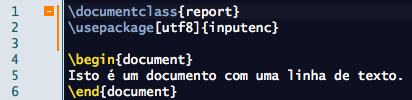
\includegraphics[width=\linewidth]{comecardocumento.png}
\end{minipage}%
\hspace*{1cm}%
\begin{minipage}{7cm}

\includegraphics[width=\linewidth]{resultadocompilacao.png}
\end{minipage}
\begin{itemize}
\aitem Compilation usually returns a .pdf file.
%\aitem If you already have an offline \LaTeX~environment ready, use it, otherwise...
\end{itemize}
\end{frame}

\note[itemize]{
		\item Dizer o que é que é o preâmbulo
		\item Voltar a apontar o inputenc
}

\subsection{Simple text editing}
\begin{frame}[t]{\textbf{bold}, \textit{italics}, \underline{underline}, \textcolor{Aquamarine}{c}\textcolor{BrickRed}{o}\textcolor{CarnationPink}{l}\textcolor{CornflowerBlue}{o}\textcolor{Lavender}{u}\textcolor{Periwinkle}{r}\textcolor{SeaGreen}{f}\textcolor{Tan}{u}\textcolor{WildStrawberry}{l}}
\begin{itemize}
\item \textcolor{blue}{$\backslash$textbf}\textcolor{PineGreen}{$\{$Bold text$\}$}
\item \textcolor{blue}{$\backslash$textit}\textcolor{PineGreen}{$\{$Italicised text$\}$}
\item \textcolor{blue}{$\backslash$underline}\textcolor{PineGreen}{$\{$Underlined text$\}$}
\item \textcolor{blue}{$\backslash$textcolor}\textcolor{PineGreen}{$\{$Colourname$\}$}$\{$Colourful text$\}$
\begin{itemize}
\item Colour names can be found here$\rightarrow$\textcolor{blue}{\url{en.wikibooks.org/wiki/LaTeX/Colors}}.
\end{itemize}
\end{itemize}
\end{frame}

\note[itemize]{
	\item Idem
}

\begin{frame}[t]{Paragraphs, line breaks and sections}
\begin{itemize}
\aitem \textcolor{blue}{$\backslash\backslash$} Breaks the line, doesn't start a new paragraph.
\aitem \textcolor{blue}{$\backslash$par} Breaks the line and starts a new paragraph.
\aitem \textcolor{blue}{$\backslash$chapter}\textcolor{PineGreen}{$\{$Chapter name$\}$} Starts a chapter.
\aitem \textcolor{blue}{$\backslash$section}\textcolor{PineGreen}{$\{$Section name$\}$} Starts a section.\\
\textcolor{blue}{$\backslash$subsection}\textcolor{PineGreen}{$\{$Subsection name$\}$},\\
\textcolor{blue}{$\backslash$subsubsection}\textcolor{PineGreen}{$\{$Subsubsection name$\}$}
\aitem All of these are numbered, writting a * before the $\{\}$ suppresses this.
\end{itemize}
\end{frame}

\note[itemize]{
	\item Esta é a maneira correcta de fazer parágrafos
	\item Tudo o que estiver a seguir a um chapter/section/etc pertence esse chapter/section/etc até o seguinte ser declarado
}

%\begin{frame}[c]{Exercício 1}
%\begin{itemize}
%\item No vosso documento, criem dois capítulos, no primeiro criem uma secção e uma subsecção não numerada.
%\end{itemize}
%\end{frame}
%
%\note[itemize]{
%	\item Dar 5 minutos, depois mostrar como
%}

\begin{frame}[t]{Titles, authors and tables of contents}
\begin{itemize}
\aitem All of these can be generated automaticaly by \LaTeX, their appearance depends on the template.
\aitem In this case, you need to give \LaTeX~the necessary information, in the preamble write:
\begin{itemize}
\bitem \textcolor{blue}{$\backslash$title}\textcolor{PineGreen}{$\{$Title$\}$}
\bitem \textcolor{blue}{$\backslash$author}\textcolor{PineGreen}{$\{$Author or Authors$\}$}
\bitem \textcolor{blue}{$\backslash$date}\textcolor{PineGreen}{$\{$Date$\}$}
\end{itemize}
\aitem For the title to appear you need to use the\textcolor{blue}{$\backslash$maketitle} command, usually right after:\\
\textcolor{blue}{$\backslash$begin}\textcolor{PineGreen}{$\{$document$\}$}
\aitem You may be given a template where the title is defined explicitly, in that case just alter the corresponding text.
\aitem To generate the index just write the command \textcolor{blue}{$\backslash$tableofcontents}, usually right after the \textcolor{blue}{$\backslash$maketitle}.
\end{itemize}
\end{frame}

\note[itemize]{
	\item Relembrar o que é que é o preâmbulo.
	\item Compilem o template que vos deram, vejam o título e procurem onde é que isso aparece no código
}

%\begin{frame}[c]{Exercício 2}
%\begin{itemize}
%\item No vosso documento, criem um título com autor e data e um índice.
%\end{itemize}
%\end{frame}

%\note[itemize]{
%	\item Dar 5 minutos, depois mostrar como
%}

\begin{frame}[t]{Changing the language of the document}
\begin{itemize}
\aitem Some compilers have a spell checker, set it to the language you are using.
\end{itemize}
\begin{minipage}{5cm}
\begin{itemize}
\aitem The language of the document can be changed with the \textcolor{PineGreen}{babel} package.
\end{itemize}
\end{minipage}%
\hspace*{1cm}%
\begin{minipage}{8cm}
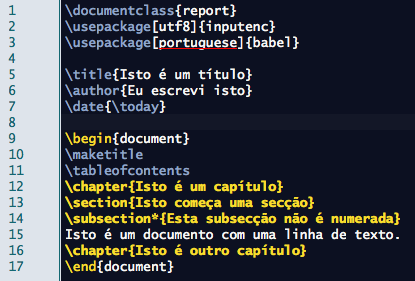
\includegraphics[width=\linewidth]{tituloeindice.png}
\end{minipage}
\end{frame}

\note[itemize]{
	\item explicar que isto muda Chapter para Capítulo, Section para Secção, etc
}

\subsection{Making tables}

\begin{frame}[t]{Tables - the hard way}
\begin{itemize}
\aitem You need to use the \textcolor{PineGreen}{$\{$table$\}$} environment.
\aitem You need to use the \textcolor{PineGreen}{$\{$tabular$\}$} environment.
\aitem You need to set the column alignment and if you want to have vertical lines between them.
\aitem You have to set the horizontal lines you want.
\end{itemize}
\textcolor{blue}{$\backslash$begin}\textcolor{PineGreen}{$\{$table$\}$}[]\\
\textcolor{blue}{$\backslash$begin}\textcolor{PineGreen}{$\{$tabular$\}$}\textcolor{PineGreen}{$\{$c$|$cl$\}$}\\
cell1 \& cell2 \& cell3 \textcolor{blue}{$\backslash\backslash$} \textcolor{blue}{$\backslash$hline}\\
cell4 \& cell5 \& cell6\\
\textcolor{blue}{$\backslash$end}\textcolor{PineGreen}{$\{$tabular$\}$}\\
\textcolor{blue}{$\backslash$end}\textcolor{PineGreen}{$\{$table$\}$}
\begin{itemize}
\aitem You can declare merged cells, partial horizontal and vertical lines, this easily becomes way too complex.
\end{itemize}
\end{frame}

\note[itemize]{
	\item Primeiro a complicada, explicar tudo
	\item Explica o código passo a passo
}

\begin{frame}[t]{Tables - the easy way}
\begin{itemize}
\aitem Use this website \textcolor{blue}{\url{www.tablesgenerator.com}}.
\end{itemize}
\begin{figure}
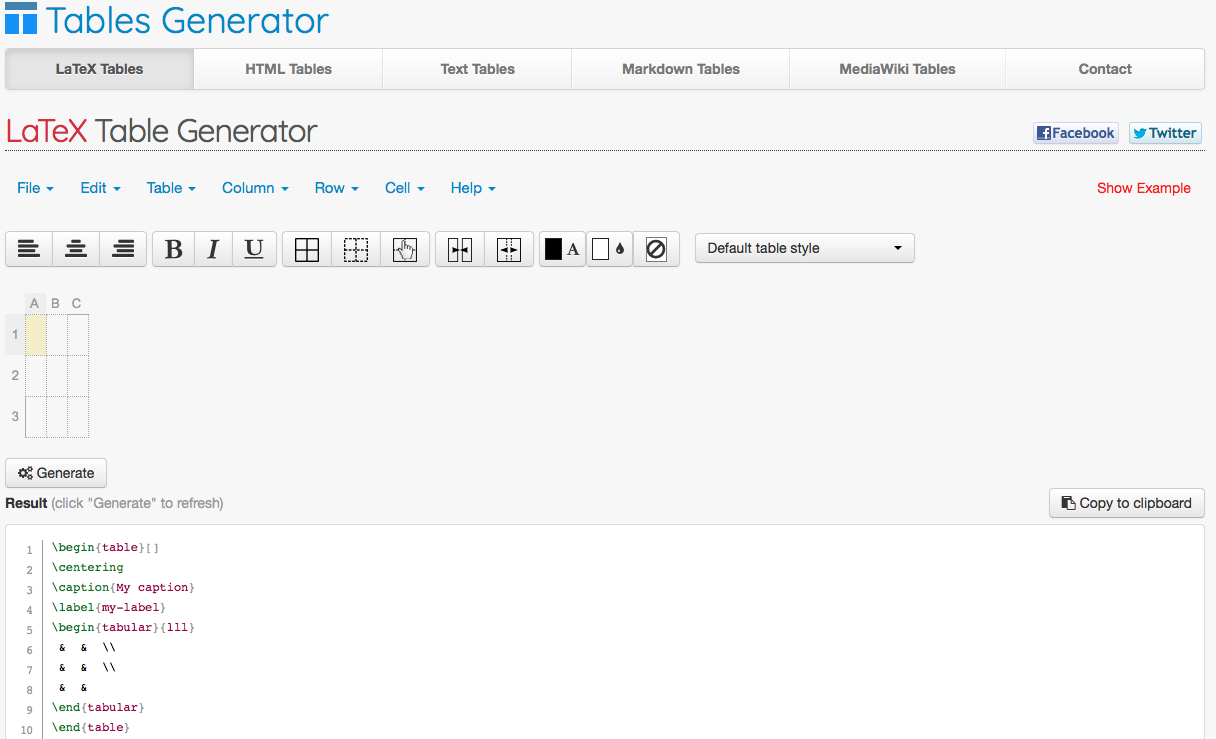
\includegraphics[width=.7\linewidth]{tablegenerator.png}
\end{figure}
\end{frame}

\note[itemize]{
	\item A maneira simples, usem esta.
	\item Funciona estilo Excell
	\item Gera o código no fim, podem copiar e colar para o documento
	\item Dá jeito perceber o método complicado, para conseguir perceber o código gerado.
}

\begin{frame}[t]{What are \textit{floats}?}
\begin{minipage}{5cm}
\begin{itemize}
\aitem You may have noticed a blank space in the previous code.
\aitem With the information inside the \textcolor{PineGreen}{[ ]}, \LaTeX~decides where it will draw the table.
\end{itemize}
\end{minipage}%
\hspace*{1cm}%
\begin{minipage}{8cm}
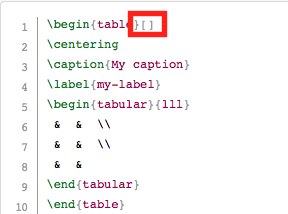
\includegraphics[width=\linewidth]{floats1.png}
\end{minipage}

\end{frame}

\note[itemize]{
	\item Chama-se um float
}

\begin{frame}[t]{Types of \textit{float}}
\begin{itemize}
\aitem There are multiple types of \textit{floats}:
\begin{itemize}
\bitem H - Draws the \textit{float} exactly where it is declared, may deform the text.
\bitem h - Draws the \textit{float} close to where it is declared, this avoids deforming the text.
\bitem t - Draws the float at the top of the page in which it is declared.
\bitem b - Draws the \textit{float} at the bottom of the page in which it is declared.
\bitem p -  Draws the float in a page restricted to \textit{floats}.
\end{itemize}
\aitem The \textcolor{PineGreen}{$\{$figure$\}$} environment also uses floats \textit{floats}.
\aitem Use the package \textcolor{PineGreen}{$\{$float$\}$}
\end{itemize}
\end{frame}

\note[itemize]{
	\item Idem
}

%\begin{frame}[c]{Exercício 3}
%\begin{itemize}
%\item Incluam no preâmbulo:
%\end{itemize}
%\textcolor{blue}{$\backslash$usepackage}\textcolor{PineGreen}{$\{$float$\}$}
%\begin{itemize}
%\item No vosso documento, criem uma tabela com:
%\begin{itemize}
%\item 3 colunas, 2 linhas.
%\item Primeira e segunda coluna centradas, terceira alinhada à esquerda.
%\item Linha vertical entre a primeira e segundas colunas.
%\item Linha horizontal entre as 2 linhas.
%\end{itemize}
%\item Usem o site que é mais fácil.
%\item Mandem desenhar no segundo capítulo.
%\item Há umas linhas de texto gerados pelo site que para já podem ignorar:
%\begin{itemize}
%\item \textcolor{blue}{$\backslash$caption}...
%\item \textcolor{blue}{$\backslash$label}...
%\item \textcolor{blue}{$\backslash$centering}
%\end{itemize}
%\end{itemize}
%\end{frame}
%
%\note[itemize]{
%	\item Dar 5 minutos, depois mostrar
%	\item linhas de caption e assim vão ser explicadas mais à frente
%	\item centering centra a tabela na página.
%}

\subsection{Figures and images}
\begin{frame}[t]{How to declare an image}
\begin{itemize}
\aitem Use the \textcolor{PineGreen}{$\{$graphicx$\}$} package.
\aitem Images need to be inside a folder where \LaTeX~knows it should look.
\end{itemize}
\textcolor{blue}{$\backslash$graphicspath}\textcolor{PineGreen}{$\{$ $\{$pathtofolder1$\}\{$pathtofolder2$\}$ $\}$}
\begin{itemize}
\aitem Images should be declared inside the \textcolor{PineGreen}{$\{$figure$\}$} environment.
\end{itemize}
\textcolor{blue}{$\backslash$begin}\textcolor{PineGreen}{$\{$figure$\}$}\textcolor{purple}{[float]}\\
\textcolor{blue}{$\backslash$centering}\\
\textcolor{blue}{$\backslash$includegraphics}\textcolor{purple}{[figure alterations]}\textcolor{PineGreen}{$\{$imagename$\}$}\\
\textcolor{blue}{$\backslash$end}\textcolor{PineGreen}{$\{$figure$\}$}
\begin{itemize}
\aitem PNG, JPG, PDF are all acepted. Other file types are as well, check google in case of doubts.
\aitem Multiple properties can be altered, check \textcolor{blue}{\url{en.wikibooks.org/wiki/LaTeX/Importing\_Graphics}}
\end{itemize}
\end{frame}

\note[itemize]{
	\item Normalmente as figuras se estiverem na mesma pasta que o .tex ele vai lá buscar tudo
	\item Podem guardar noutra(s) pasta(s), pode dar jeito para arrumar os ficheiros
	\item Nome da figura não precisa de incluir extensão, mas convém
	\item Idem
}

\subsection{Lists and enumerations}
\begin{frame}[t]{How to make a list}
\begin{itemize}
\aitem The \textcolor{PineGreen}{$\{$itemize$\}$} environment generates unnumbered lists.
\aitem The \textcolor{PineGreen}{$\{$enumerate$\}$} environment generates numbered lists.
\aitem Nested lists are very much possible.
\aitem Items are identified by the \textcolor{blue}{$\backslash$item} command.
\end{itemize}
\textcolor{blue}{$\backslash$begin}\textcolor{PineGreen}{$\{$itemize$\}$}\\
\textcolor{blue}{$\backslash$item} First item of the unnumbered list\\
\textcolor{blue}{$\backslash$begin}\textcolor{PineGreen}{$\{$enumerate$\}$}\\
\textcolor{blue}{$\backslash$item} First item of the numbered sublist\\
\textcolor{blue}{$\backslash$item} Second item of the numbered sublist\\
\textcolor{blue}{$\backslash$end}\textcolor{PineGreen}{$\{$enumerate$\}$}\\
\textcolor{blue}{$\backslash$item} Second item of the unnumbered list\\
\textcolor{blue}{$\backslash$end}\textcolor{PineGreen}{$\{$itemize$\}$}
\end{frame}

\note[itemize]{
	\item Idem
}

\subsection{Equations and other math topics}
\begin{frame}[t]{Math environments}
\begin{itemize}
\aitem Use the \textcolor{PineGreen}{$\{$amsmath$\}$} package.
\aitem \textcolor{PineGreen}{\$equation\$} generates an inline equation, can be included in the middle of a sentence.
\aitem \textcolor{PineGreen}{\$\$equation\$\$} generates a separated, centred equation.
\aitem The \textcolor{PineGreen}{$\{$equation$\}$} environment generates numbered equations, this is the best option.
\end{itemize}
\textcolor{blue}{$\backslash$begin}\textcolor{PineGreen}{$\{$equation$\}$}\\
\textcolor{PineGreen}{equation}\\
\textcolor{blue}{$\backslash$end}\textcolor{PineGreen}{$\{$equation$\}$}
\begin{itemize}
\aitem A blank line inside a math environment causes a compilation error!
\end{itemize}
\end{frame}

\note[itemize]{
	\item Há vários ambientes matemáticos
	\item Há vários packages
	\item o \textit{amsmath} tem tudo o que precisam normalmente
	\item \$\$coisa\$\$ é parecido com o ambiente equation, mas não é numerado
	\item o ambiente é melhor
}

\begin{frame}[t]{Greek letters and other special symbols}
\begin{itemize}
\aitem You need to use the letter names in english.
\begin{itemize}
\bitem \textcolor{blue}{$\backslash$alpha} writes $\alpha$.
\bitem \textcolor{blue}{$\backslash$beta} writes $\beta$.
\bitem etc
\end{itemize}
\aitem There are arrows and mathematical symbols
\begin{itemize}
\bitem \textcolor{blue}{$\backslash$rightarrow} writes $\rightarrow$.
\bitem \textcolor{blue}{$\backslash$simeq} writes $\simeq$.
\bitem etc
\end{itemize}
\aitem All of these symbols can only be used in a math environment.
\aitem Check the list here \textcolor{blue}{\url{en.wikibooks.org/wiki/LaTeX/Mathematics}}
\end{itemize}
\end{frame}

\note[itemize]{
	\item Se quiserem usar um destes símbolos numa frase têm de usar os \$
}

\begin{frame}[t]{Fractions, parentheses and square roots}
\begin{itemize}
\aitem Inside a math environment, it's declared as:
\end{itemize}
\textcolor{blue}{$\backslash$frac}\textcolor{PineGreen}{$\{$numerator$\}$}\textcolor{PineGreen}{$\{$denominator$\}$}
\begin{itemize}
\aitem You can have a parentheses with necessary size to envelop the fraction:
\end{itemize}
\textcolor{blue}{$\backslash$left(}\textcolor{blue}{$\backslash$frac}\textcolor{PineGreen}{$\{$numerator$\}$}\textcolor{PineGreen}{$\{$denominator$\}$}\textcolor{blue}{$\backslash$right)}
\begin{itemize}
\aitem This method for parentheses works with [, $\{$ e ``.''.
\aitem Using \textcolor{blue}{$\backslash$left.}\textcolor{PineGreen}{something}\textcolor{blue}{$\backslash$right)} causes only the right parenthesis to be drawn.
\aitem Having a mismatched number of \textcolor{blue}{$\backslash$left} or \textcolor{blue}{$\backslash$right} causes a compilation error!
\aitem Roots envelop the whole radicand:
\end{itemize}
\textcolor{blue}{$\backslash$sqrt}\textcolor{purple}{[index]}\textcolor{PineGreen}{$\{$radicand$\}$}
\end{frame}

\note[itemize]{
	\item Explicar o que é o $\backslash$left.
	\item Por cada left é preciso um right
	\item se não se meter o índice é uma raiz quadrada sem nada
}

\begin{frame}[t]{Superscripts, subscripts, vectors and accents}
\begin{itemize}
\aitem The $\hat{}$ symbol puts things in superscript, this is how you write powers.
\end{itemize}
\textcolor{PineGreen}{basis$\hat{}\{$exponent$\}$} $\Rightarrow$ $\text{basis}^\text{exponent}$
\begin{itemize}
\aitem The \_ symbol puts things in subscript, this is how you write indices.
\end{itemize}
\textcolor{PineGreen}{basis\_$\{$subscript$\}$} $\Rightarrow$ $\text{basis}_\text{subscript}$
\begin{itemize}
\aitem Vectors are declared by the $\backslash vec\{\}$ command.
\end{itemize}
\textcolor{PineGreen}{$\backslash vec\{v\}$} $\Rightarrow$ $\vec{v}$
\begin{itemize}
\aitem For more, see \textcolor{blue}{\url{en.wikibooks.org/wiki/LaTeX/Mathematics}}
\end{itemize}
\end{frame}

\note[itemize]{
	\item Usar o $\hat{}$ ou o \_ fora de ambiente matemático causa erro
}

%\begin{frame}[c]{Exercício 4}
%\begin{itemize}
%\item Incluam no preâmbulo:
%\end{itemize}
%\textcolor{blue}{$\backslash$usepackage}\textcolor{PineGreen}{$\{$amsmath$\}$}
%\begin{itemize}
%\item No vosso documento, criem uma equação numerada com o conteúdo $\gamma=\frac{1}{\sqrt{1-\left(\frac{v}{c}\right)^2}}$.
%\item No vosso documento escrevam a frase "O ângulo resultante é $\alpha=\frac{\pi}{2}$."
%\end{itemize}
%\end{frame}
%
%\note[itemize]{
%	\item Mostrar onde está a lista de letras gregas no texmaker
%	\item Mostrar a lista de letras gregas no site
%	\item Dar 5 minutos, depois mostrar como se faz
%}



%\begin{frame}[c]{Exercício 5}
%\begin{itemize}
%\item Incluam no preâmbulo:
%\end{itemize}
%\textcolor{blue}{$\backslash$usepackage}\textcolor{PineGreen}{$\{$graphicx$\}$}
%\begin{itemize}
%\item No vosso documento, criem uma figura com a imagem que vos foi fornecida, com largura igual a metade da largura da linha.
%\end{itemize}
%\end{frame}
%
%\note[itemize]{
%	\item Dar 5 minutos, depois mostrar
%}

\subsection{Referencing content}
\begin{frame}[t]{What is a reference?}
\begin{itemize}
\aitem To call, by a number, some equation, figure or table.
\aitem There are 3 different commands for this:
\begin{itemize}
\bitem \textcolor{blue}{$\backslash$label}\textcolor{PineGreen}{$\{$identificationtext$\}$}
\bitem \textcolor{blue}{$\backslash$ref}\textcolor{PineGreen}{$\{$identificationtext$\}$}
\bitem \textcolor{blue}{$\backslash$eqref}\textcolor{PineGreen}{$\{$equationidentificationtext$\}$}
\end{itemize}
\aitem You can call the reference before and after it appears in the text.
\aitem \LaTeX deals with the pesky problem of numbering.
\end{itemize}
\end{frame}

\note[itemize]{
	\item Uma das grandes vantagens é o sistema de numeração, funciona bem
	\item Numeração é por ordem que são declarados
	\item Normalmente é preciso compilar 2x para as referências funcionarem depois de serem declaradas pela primeira vez ou serem alteradas. Tem a ver com os ficheiros auxiliares
}

\begin{frame}[t]{Referencing equations}
\begin{itemize}
\aitem Just add a label to the equation:
\end{itemize}
\textcolor{blue}{$\backslash$begin}\textcolor{PineGreen}{$\{$equation$\}$}\textcolor{YellowOrange}{$\backslash$label$\{$labeltext$\}$}\\
\textcolor{PineGreen}{equation content}\\
\textcolor{blue}{$\backslash$end}\textcolor{PineGreen}{$\{$equation$\}$}
\begin{itemize}
\aitem You then call the reference with the \textcolor{blue}{$\backslash$eqref} command:
\end{itemize}
"As demonstrated in relation \textcolor{blue}{$\backslash$eqref}\textcolor{PineGreen}{$\{$labeltext$\}$}..."
\begin{itemize}
\aitem This command is made especially for equations, the reference appears between parenthesis.
\end{itemize}
\end{frame}

\note[itemize]{
	\item idem
}

\begin{frame}[t]{Referenciar tabelas e figuras}
\begin{itemize}
\aitem The figure/table needs to have a caption.
\aitem Just add a label to the figure/table.
\end{itemize}
\textcolor{blue}{$\backslash$begin}\textcolor{PineGreen}{$\{$table$\}$}[]\\
\textcolor{blue}{$\backslash$caption}\textcolor{PineGreen}{$\{$legend$\}$}\\
\textcolor{YellowOrange}{$\backslash$label$\{$labeltext$\}$}\\
\textcolor{blue}{$\backslash$begin}\textcolor{PineGreen}{$\{$tabular$\}$}\textcolor{PineGreen}{$\{$c$|$cl$\}$}\\
Table content...\\
\textcolor{blue}{$\backslash$end}\textcolor{PineGreen}{$\{$tabular$\}$}\\
\textcolor{blue}{$\backslash$end}\textcolor{PineGreen}{$\{$table$\}$}
\begin{itemize}
\aitem You then call the reference with the \textcolor{blue}{$\backslash$ref} command.
\aitem Usually, table captions are placed above the table.
\end{itemize}
\end{frame}

\note[itemize]{
	\item idem
}

\begin{frame}[t]{Referenciar tabelas e figuras}
\begin{itemize}
\aitem The figure/table needs to have a caption.
\aitem Just add a label to the figure/table.
\end{itemize}
\textcolor{blue}{$\backslash$begin}\textcolor{PineGreen}{$\{$figure$\}$}\textcolor{purple}{[float]}\\
\textcolor{blue}{$\backslash$centering}\\
\textcolor{blue}{$\backslash$includegraphics}\textcolor{purple}{[...]}\textcolor{PineGreen}{$\{$imagename$\}$}\\
\textcolor{blue}{$\backslash$caption}\textcolor{PineGreen}{$\{$legend$\}$}\\
\textcolor{YellowOrange}{$\backslash$label$\{$labeltext$\}$}\\
\textcolor{blue}{$\backslash$end}\textcolor{PineGreen}{$\{$figure$\}$}
\begin{itemize}
\aitem You then call the reference with the \textcolor{blue}{$\backslash$ref} command.
\end{itemize}
\end{frame}

\note[itemize]{
	\item idem
}

%\begin{frame}[c]{Exercício 6}
%\begin{itemize}
%\item No vosso documento, adicionem rótulos à tabela, equação e figura e referenciem numa frase.
%\item Lembrem-se que precisam de adicionar uma legenda à figura e à tabela.
%\end{itemize}
%\end{frame}
%
%\note[itemize]{
%	\item Dar 5 minutos, depois mostrar
%	\item Usar referências com eq: fig: tabl:, explicar que dá jeito rotular os rótulos
%}

\subsection{Bibliographies and citations}
\begin{frame}[t]{How to make a bibliography}
\begin{itemize}
\aitem Easiest way is to have a .bib file.
\aitem This file can be made by hand or with a reference management software (Mendeley, Bibdesk or other).
\aitem I'll show you how to do it by hand.
\aitem Generate a .bib file, somehow, by changing the extension of a .txt  created with notepad, for example.
\aitem Go get the reference text and copy it into the .bib file.
\end{itemize}
\end{frame}

\note[itemize]{
	\item Podem declarar a bibliografia dentro do .tex, mas assim é mais fácil
	\item Agora mostrovos onde ir buscar um texto de referência facilmente
}

\begin{frame}[t]{Where to get references}
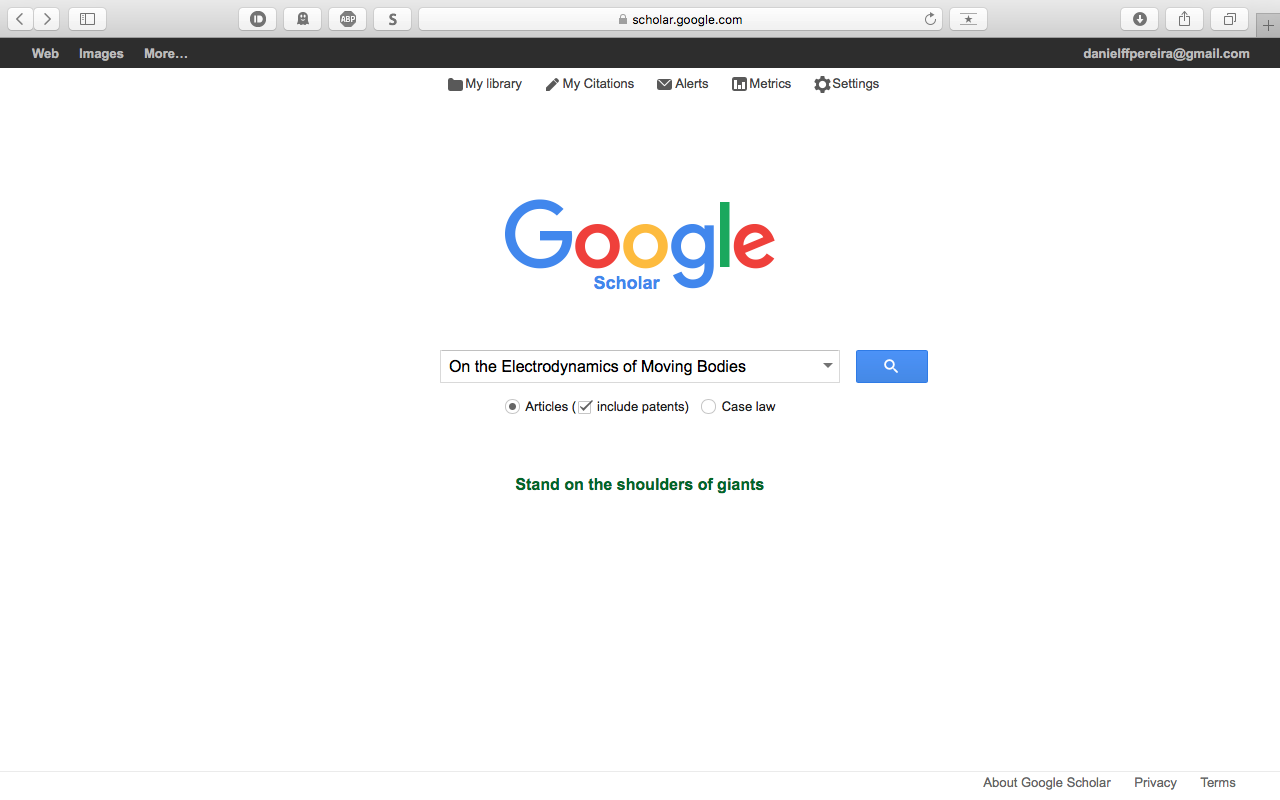
\includegraphics[trim={0 10cm 0 0}, clip=true, width=\linewidth]{biblio1.png}
\end{frame}

\begin{frame}[t]{Where to get references}
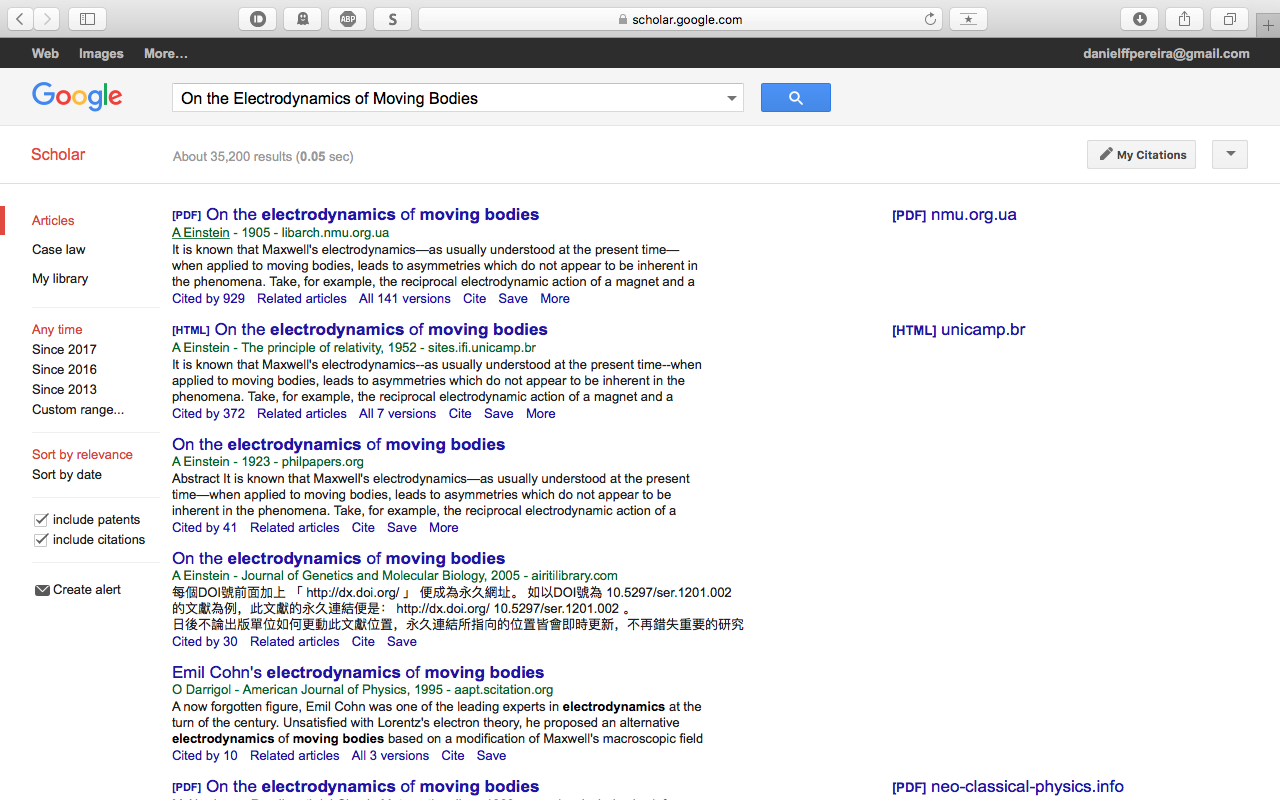
\includegraphics[trim={0 10cm 0 0}, clip=true, width=\linewidth]{biblio2.png}
\end{frame}

\begin{frame}[t]{Where to get references}
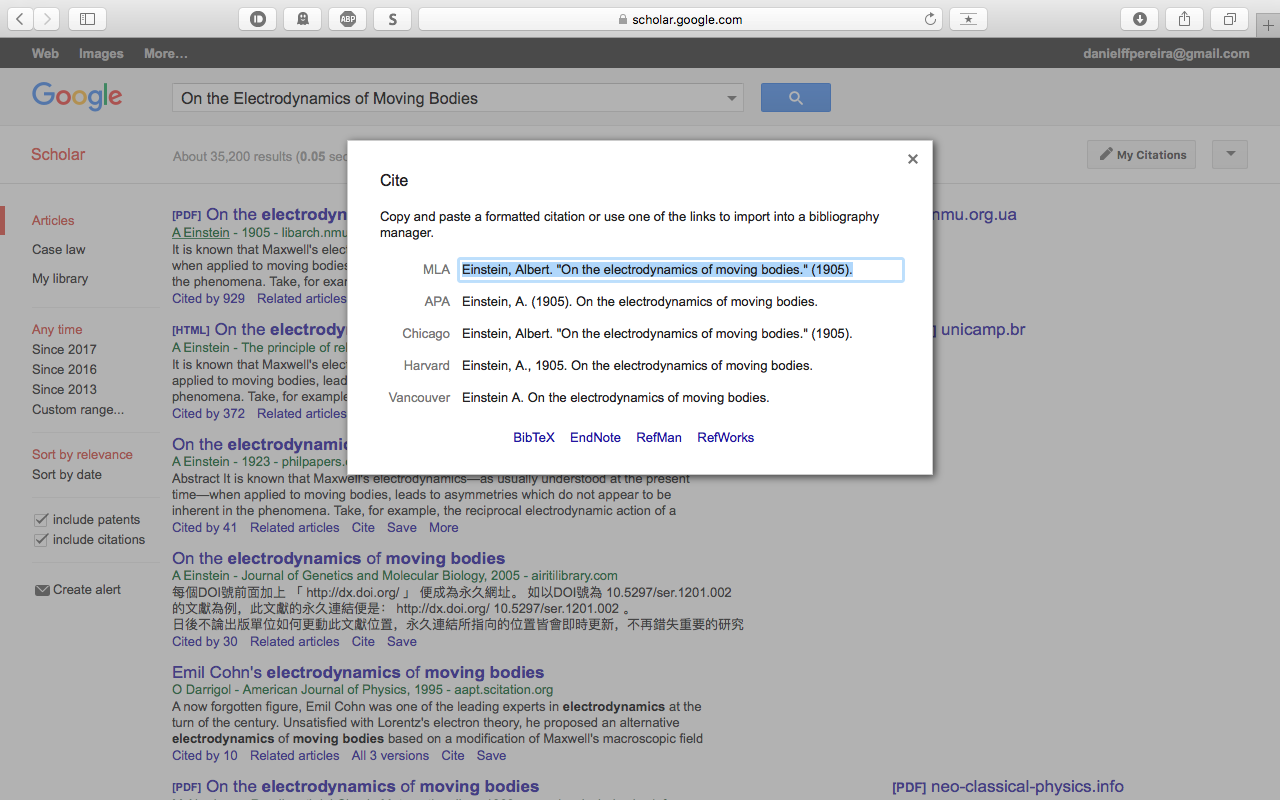
\includegraphics[trim={0 10cm 0 0}, clip=true, width=\linewidth]{biblio3.png}
\end{frame}

\begin{frame}[t]{Where to get references}
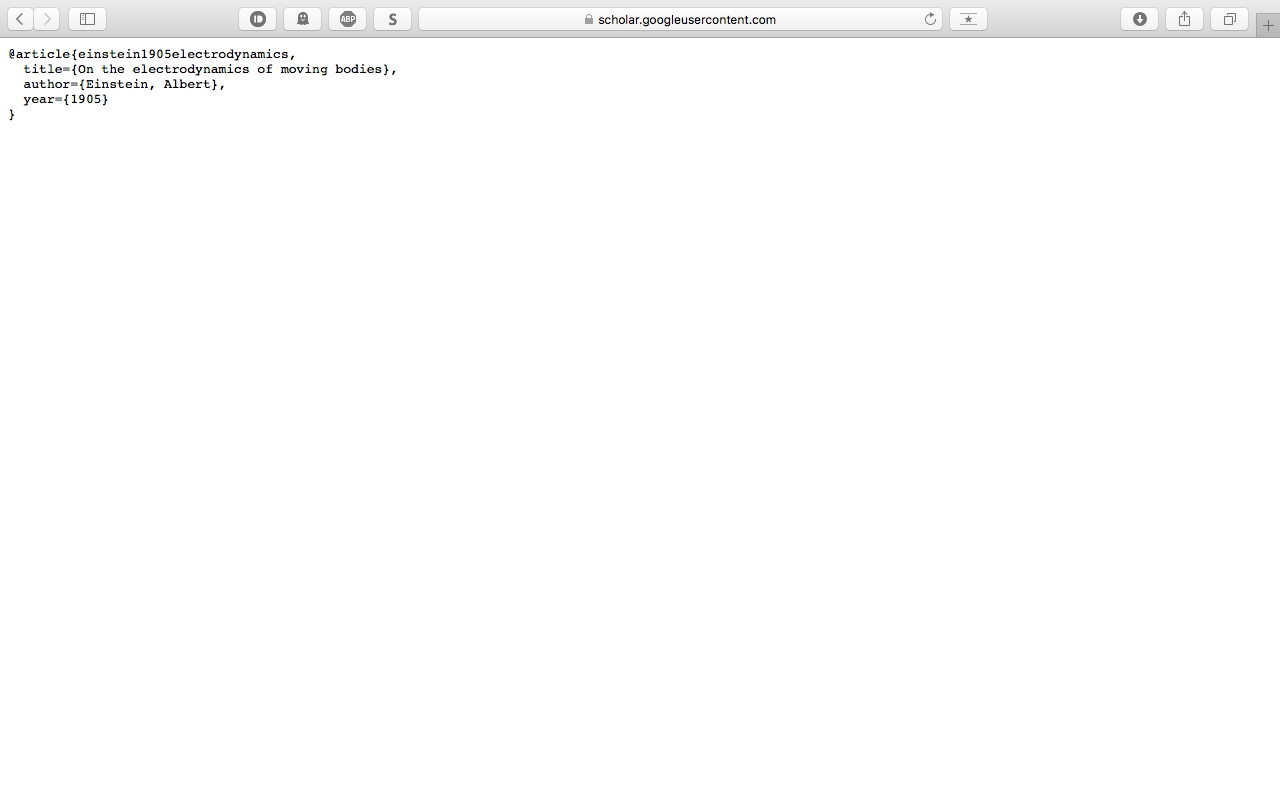
\includegraphics[trim={0 10cm 0 0}, clip=true, width=\linewidth]{biblio4.png}
\end{frame}

% trim={<left> <lower> <right> <upper>}

\begin{frame}[t]{Understanding the citation text}
\textcolor{YellowOrange}{@article$\{$}einstein1905electrodynamics,\\
\textcolor{purple}{~~~title=$\{$On the electrodynamics of moving bodies$\}$,\\
~~~author=$\{$Einstein, Albert$\}$,\\
~~~year=$\{$1905$\}$\\}
\textcolor{YellowOrange}{$\}$}
\begin{itemize}
\aitem Different publications want different formats.
\end{itemize}
\textcolor{YellowOrange}{@typeofsource$\{$}citetext,\\
\textcolor{purple}{~~~title=$\{$Source title$\}$,\\
~~~author=$\{$Authors$\}$,\\
~~~year=$\{$Publication year$\}$\\}
\textcolor{YellowOrange}{$\}$}
\end{frame}

\note[itemize]{
	\item Há muitas mais informações que podem vir com a referência
	\item Podem por exemplo querer só a inicial do primeiro nome dos autores.
}

\begin{frame}[t]{How to insert the bibliography in the document}
\begin{itemize}
\aitem After preparing a .bib file, you need to feed it to \LaTeX.
\end{itemize}
\textcolor{blue}{$\backslash$bibliography}\textcolor{PineGreen}{$\{$bibliography$\}$}
\begin{itemize}
\aitem There are different styles of bibliographies, they change the way things are presented.
\end{itemize}
\textcolor{blue}{$\backslash$bibliographystyle}\textcolor{PineGreen}{$\{$plain$\}$}
\begin{itemize}
\aitem By default, \LaTeX only includes cited sources in the bibliography, if you want uncited sources to be included, use the code:
\end{itemize}
\textcolor{blue}{$\backslash$nocite}\textcolor{PineGreen}{$\{$*$\}$}
\end{frame}

\note[itemize]{
	\item idem
	\item há vários estilos, se o texto está em itálico por exemplo.
	\item só têm de se preocupar com o style se forem escrever para uma revista
}

\begin{frame}[t]{How to cite a source}
\begin{itemize}
\aitem After having included the bibliography in the document, this is cited with the \textcolor{blue}{$\backslash$cite}\textcolor{PineGreen}{$\{$citetext$\}$} command.
\aitem If you wish to cite multiple sources at the same time, do:
\end{itemize}
\textcolor{blue}{$\backslash$cite}\textcolor{PineGreen}{$\{$citetext1,citetext2,citetext3,...$\}$}
\begin{itemize}
\aitem For more, see \textcolor{blue}{\url{en.wikibooks.org/wiki/LaTeX/Bibliography\_Management}}
\end{itemize}
\end{frame}

\note[itemize]{
	\item idem
}

\subsection{This concludes the \LaTeX mini-workshop}
\note[itemize]{
	\item Any questions
}

\section{Introduction to Git}
\subsection{Intro}
\begin{frame}[t]{Initial notions}
\begin{itemize}
\aitem What is it?
\begin{itemize}
\bitem A database control and sharing system.
\end{itemize}
\aitem GitHub is a very popular option, it's free and open. Create an account on GitHub.
\aitem You need to install the git distribution.
\begin{itemize}
\bitem Windows: \textcolor{blue}{\url{gitforwindows.org}}
\bitem Mac: \textcolor{blue}{\url{sourceforge.net/projects/git-osx-installer/files/}}
\bitem Linux: run the following code in the console (this should work for most distros)
\end{itemize}
\end{itemize}
\textcolor{purple}{
sudo apt-get update\\
sudo apt-get install git}
\begin{itemize}
\aitem You can use a Git client (or work directly in the console):
\begin{itemize}
\bitem GitKraken: \textcolor{blue}{\url{www.gitkraken.com/git-client}}
\bitem GitHub Desktop: \textcolor{blue}{\url{desktop.github.com}}
\end{itemize}
\end{itemize}
\end{frame}

\note[itemize]{
	\item Git actually can run from the command line
	\item Using it that way is not a good idea for beginners
	\item You are going to use GitHub, so use GitHub Desktop client
	\item The practical explanations presented in the rest of this workshop assume you are using GitHub Desktop client
	\item SO USE OTHER CLIENTS AT YOUR OWN RISK
}

\begin{frame}[t]{What is a repository}
\begin{itemize}
\aitem A repository is a data structure that:
\begin{itemize}
\bitem Stores a set of files and/or a directory structure.
\bitem A historical record of the changes to those files.
\end{itemize}
\aitem The main repository lives somewhere in a server.
\aitem You can \textbf{clone} a copy of the repository to your PC.
\aitem Changes are made locally to the cloned repository can be made permanent by \textbf{committing} to it.
\aitem Changes can then be \textbf{pushed} to the external repository.
\aitem If you are working on another computer, you can then \textbf{pull} the changes from the external repository.
\end{itemize}
\end{frame}

\note[itemize]{
	\item Similar to Dropbox or OneDrive, but it only uploads when you tell it to
	\item Read slide and explain line by line
	\item For the work in this class you will be working on a repository that already exists, but it belongs to someone else, so... NEXT SLIDE
}

\subsection{Forking repositories}
\begin{frame}[t]{What the fork?}
\begin{itemize}
\aitem A fork is a copy of another repository.
\aitem In the GitHub website, navigate to the repository you want to fork.
\end{itemize}
\begin{figure}
\centering

\includegraphics[width=\linewidth]{forking1}
\end{figure}
\end{frame}

\note[itemize]{
	\item A fork is a copy of someone's repository to your account
	\item You can't change someone else's repository directly, but you can change your fork of it as much as you want
	\item Click on the Fork button and... NEXT SLIDE
}

\begin{frame}[t]{How to fork a repository}% What the fork?
\begin{itemize}
\aitem A fork is a copy of another repository.
\aitem In the GitHub website, navigate to the repository you want to fork.
\end{itemize}
\begin{figure}
\centering

\includegraphics[width=\linewidth]{forking1}

\includegraphics[width=\linewidth]{forking2}
\end{figure}
\end{frame}

\note[itemize]{
	\item This is your fork
	\item Point out the usernames in the figure
	\item Now you want to work on your fork, alter files and such, so you... NEXT SLIDE
}

\begin{frame}[t]{How to clone your fork}% Git wars: the clone wars
\begin{minipage}{5cm}
\begin{itemize}
\aitem This is not the only way to do it, but it is the easiest.
\aitem In the GitHub Desktop app, choose to \textit{clone a repository}.
\end{itemize}
\end{minipage}%
\hspace{.5cm}%
\begin{minipage}[*]{8cm}
\begin{figure}
\centering
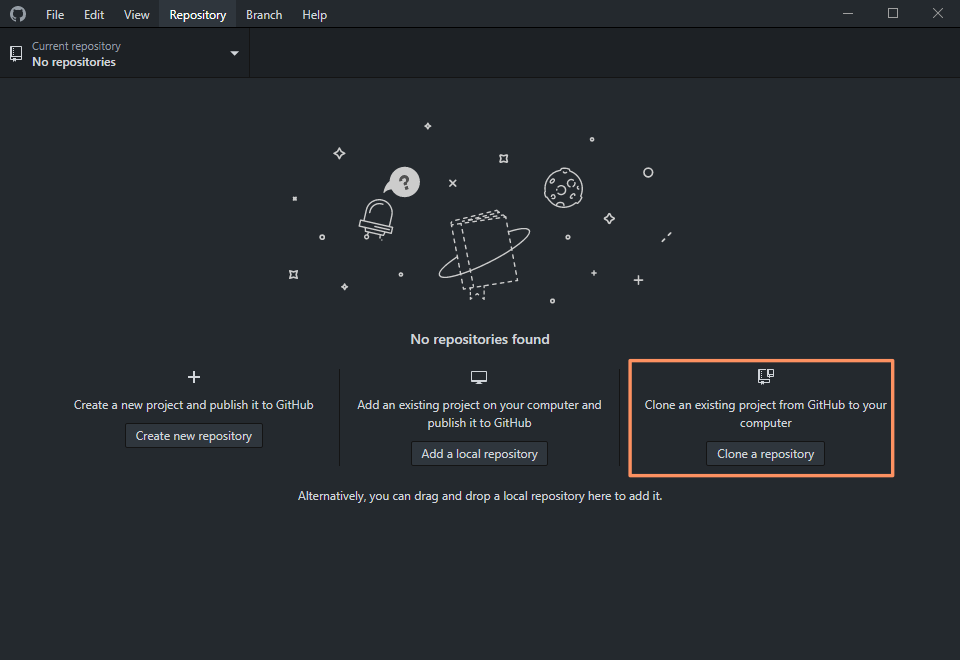
\includegraphics[width=\linewidth]{cloning1}
\end{figure}
\end{minipage}
\end{frame}

\note[itemize]{
	\item ... clone your fork to your machine
	\item you can do this in multiple ways, do it this way to be simpler
	\item click on clone a repository... NEXT SLIDE
}

\begin{frame}[t]{How to clone your fork}% Git wars: the clone wars
\begin{minipage}{5cm}
\begin{itemize}
\aitem This is not the only way to do it, but it is the easiest.
\aitem In the GitHub Desktop app, choose to \textit{clone a repository}.
\end{itemize}
\end{minipage}%
\hspace{.5cm}%
\begin{minipage}[*]{8cm}
\begin{figure}
\centering
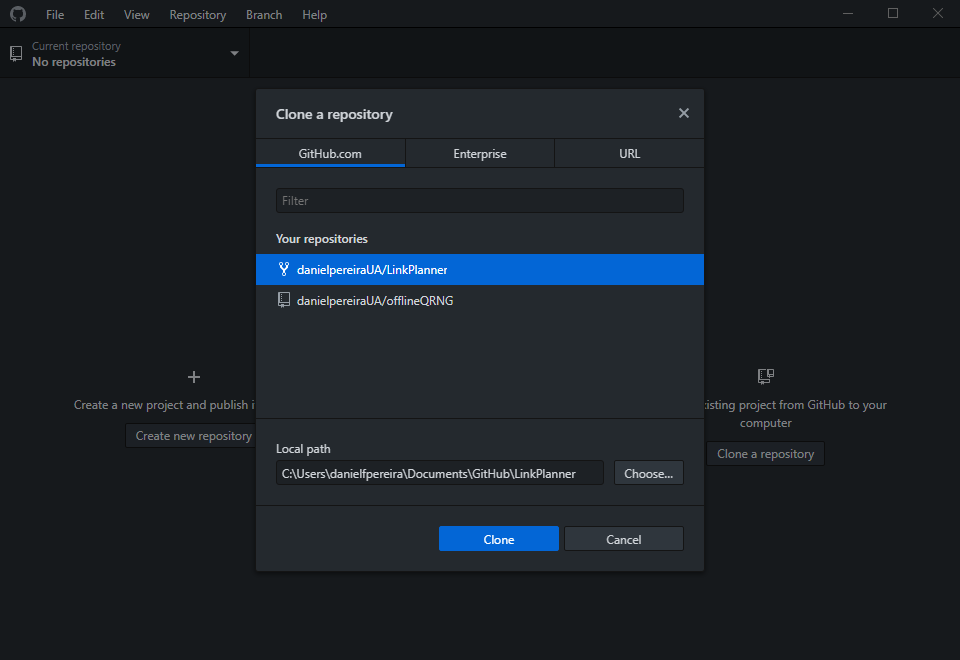
\includegraphics[width=\linewidth]{cloning2}
\end{figure}
\end{minipage}
\end{frame}

\note[itemize]{
	\item this shows a list of the repositories associated to your GitHub account
	\item point out they can choose the path to where it will download the files
	\item choose the one you want to clone and... NEXT SLIDE
}

\begin{frame}[t]{How to clone your fork}% Git wars: the clone wars
\begin{minipage}{5cm}
\begin{itemize}
\aitem This is not the only way to do it, but it is the easiest.
\aitem In the GitHub Desktop app, choose to \textit{clone a repository}.
\aitem Then you just have wait while it downloads, may take a while.
\end{itemize}
\end{minipage}%
\hspace{.5cm}%
\begin{minipage}[*]{8cm}
\begin{figure}
\centering
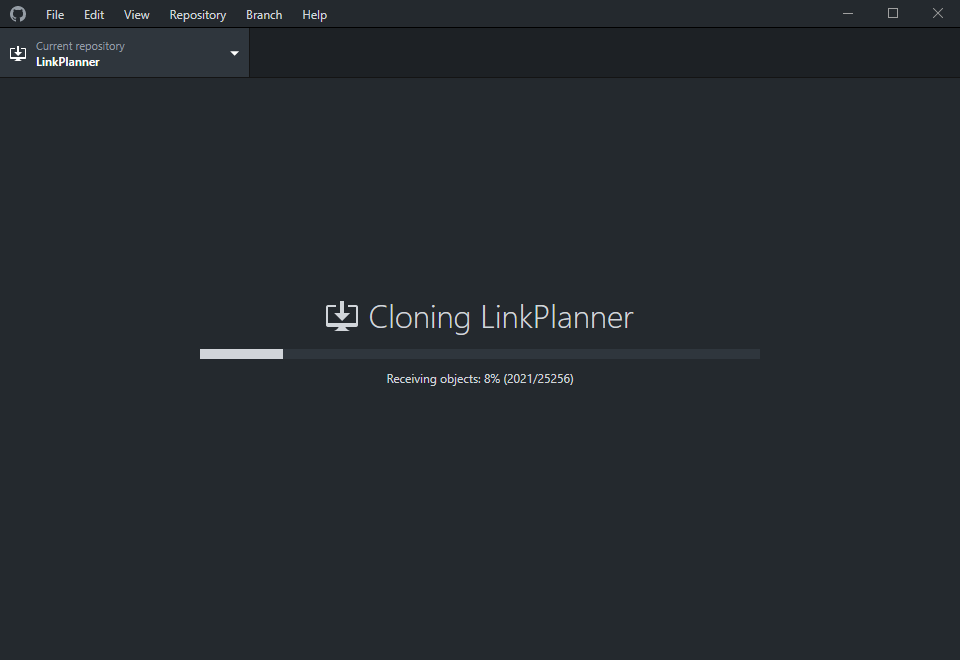
\includegraphics[width=\linewidth]{cloning3}
\end{figure}
\end{minipage}
\end{frame}

\note[itemize]{
	\item just wait
}

\subsection{Working inside your fork}
\begin{frame}[t]{Branches}
\begin{itemize}
\aitem What is a branch?
\begin{itemize}
\bitem You can see it as a split of a repository inside it.
\bitem While a fork is to another account, a branch remains in the same account.
\bitem Allows code to be tested before it is included in the main branch.
\end{itemize}
\aitem You won't have to worry about branches much in this class, only that you \underline{work on the branch allotted to you}.
\end{itemize}
\end{frame}

\note[itemize]{
	\item before you do anything, make sure you are working on the branch allotted to you
}

\begin{frame}[t]{Branches}
\begin{figure}
\centering
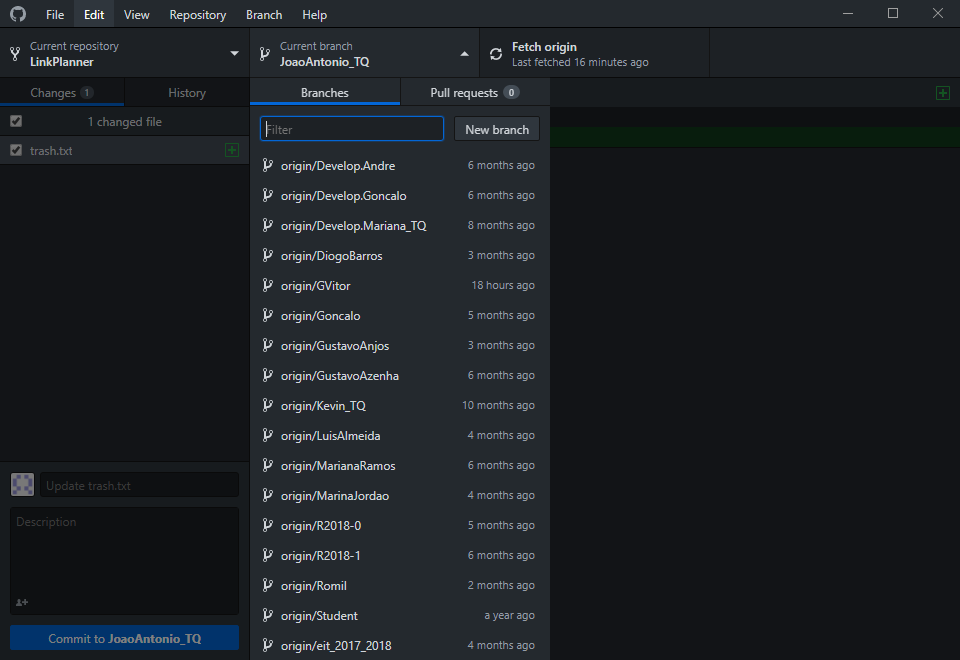
\includegraphics[width=.7\linewidth]{branches}
\end{figure}
\end{frame}

\note[itemize]{
	\item before you do anything, make sure you are working on the branch allotted to you
	\item there are only branches with origin/... in the branch name means that it is not yet listed on your fork however... NEXT SLIDE
}

\begin{frame}[t]{Branches}
\begin{figure}
\centering
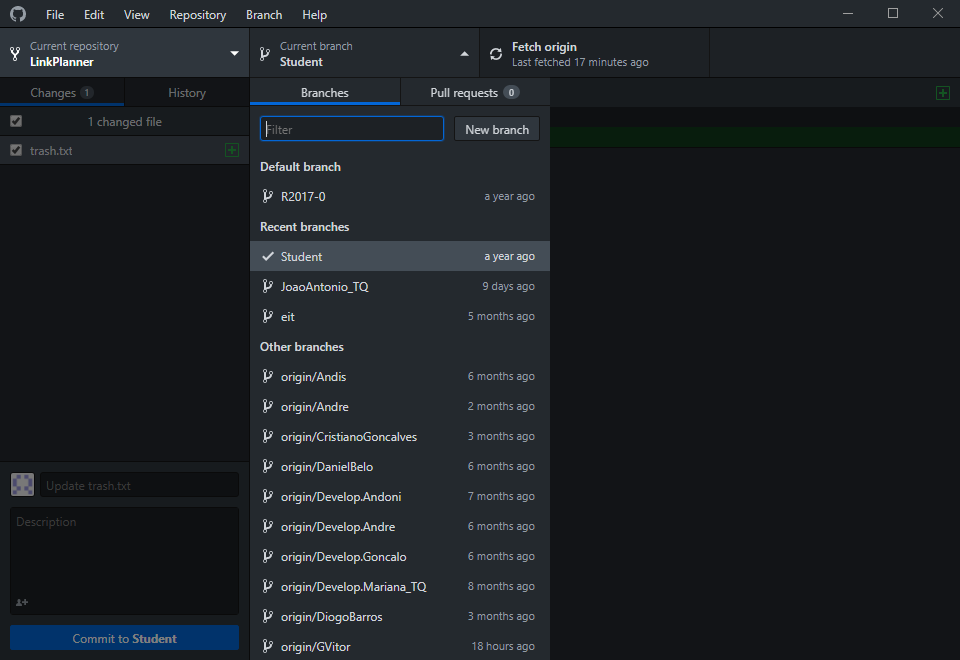
\includegraphics[width=.7\linewidth]{branches2}
\end{figure}
\end{frame}

\note[itemize]{
	\item after the first selection, it is included in your fork, use this version from then on
}

\begin{frame}[t]{Committing, pushing and pulling}
\begin{minipage}{8cm}
\begin{itemize}
\aitem Alterations made on your \textbf{clone} (that lives on your computer) can be made ``official'' by \textit{committing} to them.
\aitem You can discard changes by \textit{checking out} the version of the latest commit. You can even \textbf{check out} a version of a file from any previous commit.
\aitem The alterations you make this way are local to your machine, you need to \textbf{push} them to your ``cloud'' repository.
\aitem If you wish to work on your repository on another machine, you will need to \textbf{pull} the latest version from the ``cloud'' repository.
\end{itemize}
\end{minipage}%
\hspace{.5cm}%
\begin{minipage}[*]{5.5cm}
\begin{figure}
\centering
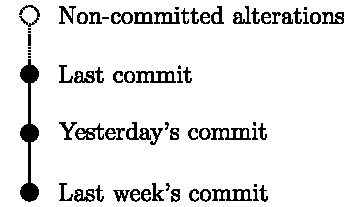
\includegraphics[width=\linewidth]{commitTopology}
\end{figure}
\end{minipage}
\end{frame}

\note[itemize]{
	\item You can now freely work on your clone of your fork of the original repository
	\item Checking out files from previous commits is not the easiest thing you can do, don't do it lightly.
}

\begin{frame}[t]{Committing, pushing and pulling}
\begin{figure}
\centering
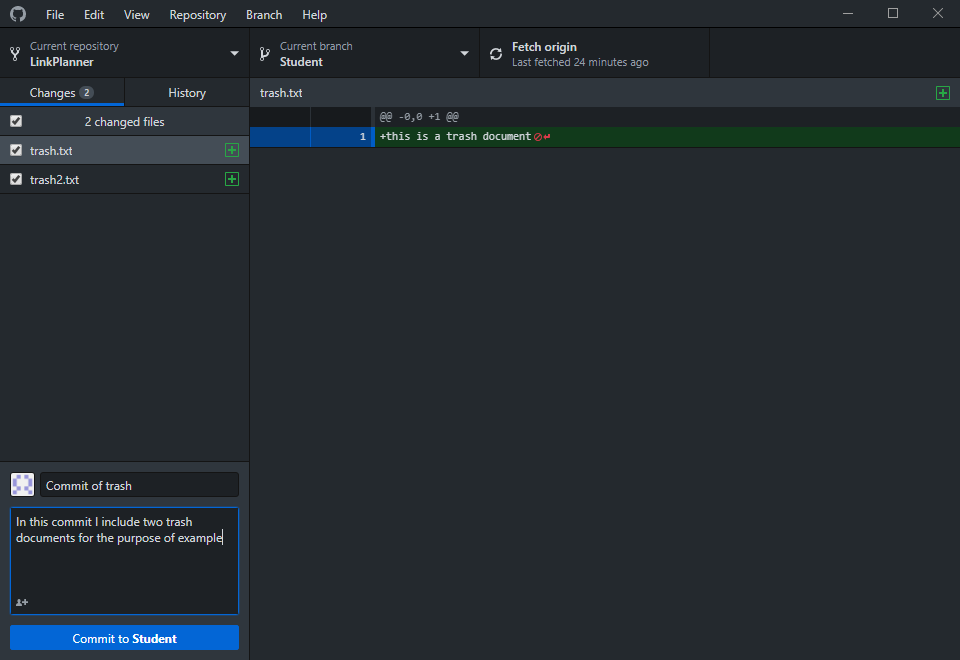
\includegraphics[width=.7\linewidth]{committing1}
\end{figure}
\end{frame}

\note[itemize]{
	\item here I have 2 different changes that I haven't committed yet
	\item You need to write a summary (point to it) and a description of the changes you made.
	\item After that click commit.
}

\begin{frame}[t]{Committing, pushing and pulling}
\begin{figure}
\centering
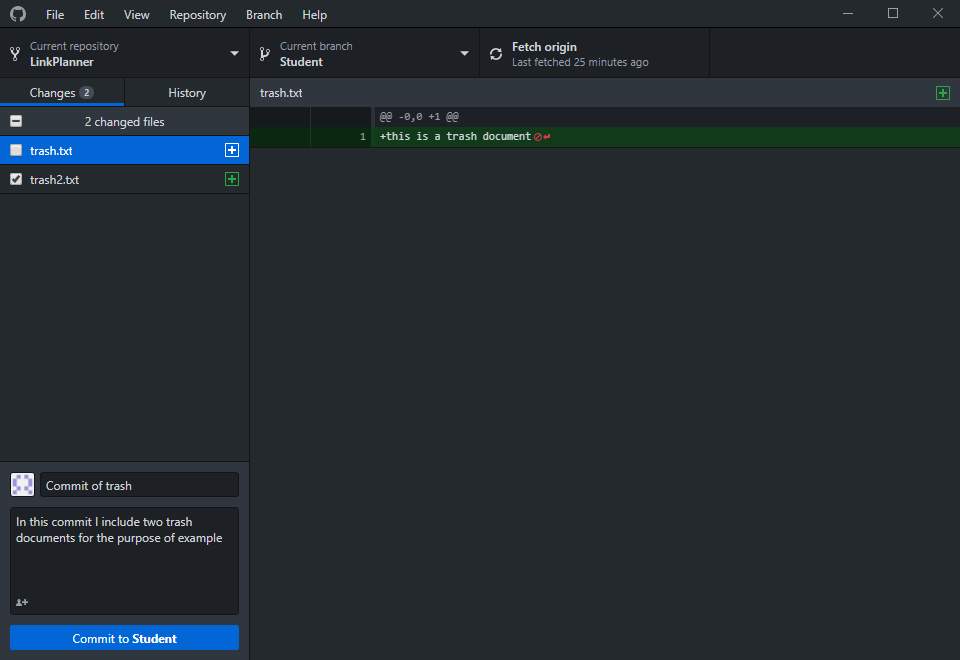
\includegraphics[width=.7\linewidth]{committing2}
\end{figure}
\end{frame}

\note[itemize]{
	\item I can choose not to include some files in the commit, these can be committed at a later stage or discarded.
	\item Point to the checkmarks.
}

\begin{frame}[t]{Committing, pushing and pulling}
\begin{figure}
\centering
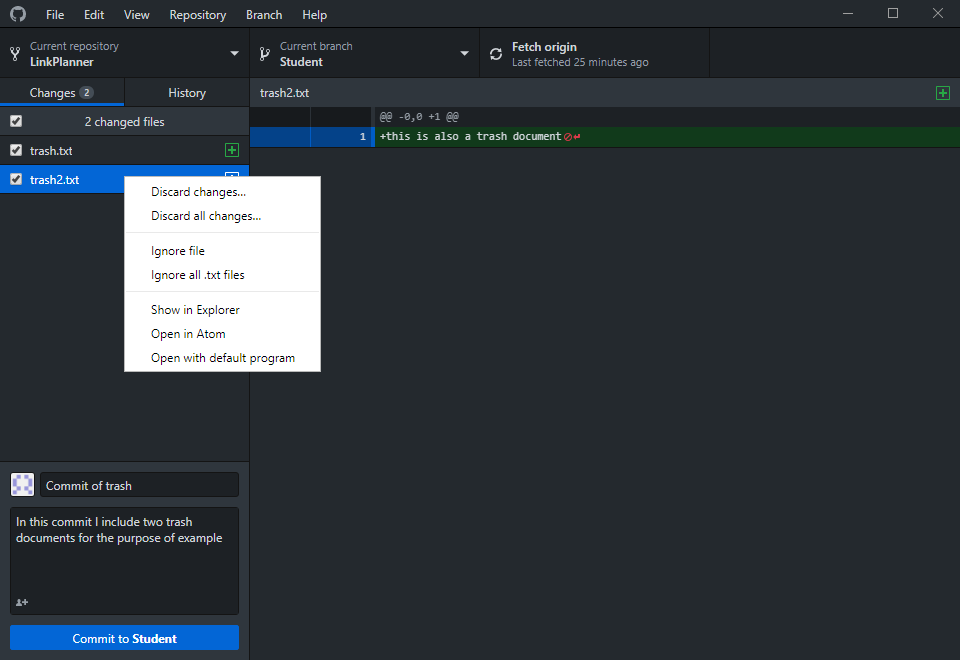
\includegraphics[width=.7\linewidth]{committing3}
\end{figure}
\end{frame}

\note[itemize]{
	\item The discarding options appear if you right click the changes.
}

\begin{frame}[t]{Committing, pushing and pulling}
\begin{figure}
\centering
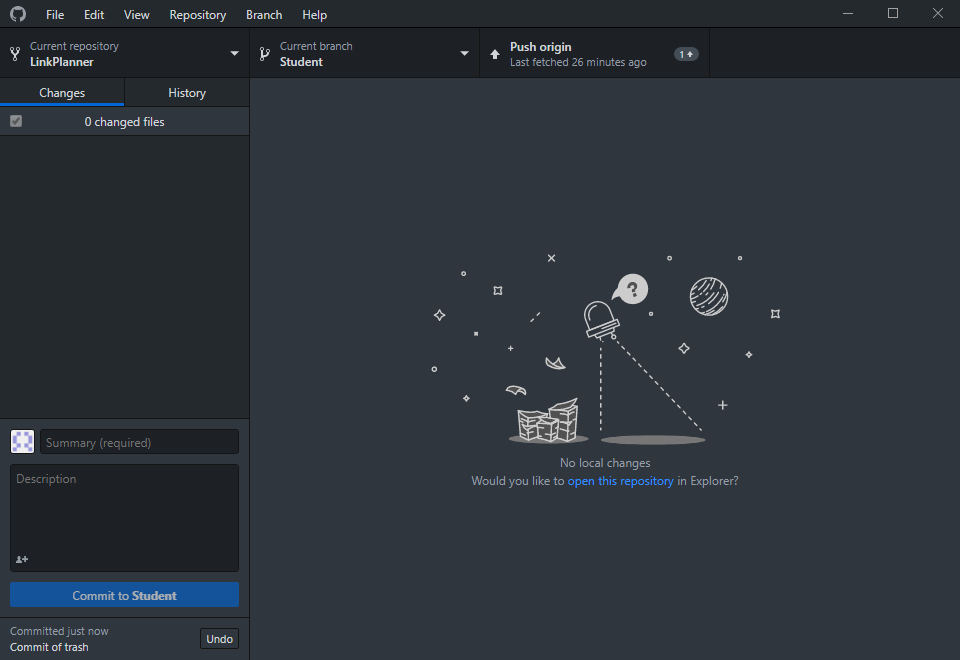
\includegraphics[width=.7\linewidth]{committing4}
\end{figure}
\end{frame}

\note[itemize]{
	\item After you commit, you need to push those changes to the cloud... NEXT SLIDE
}

\begin{frame}[t]{Committing, pushing and pulling}
\begin{figure}
\centering
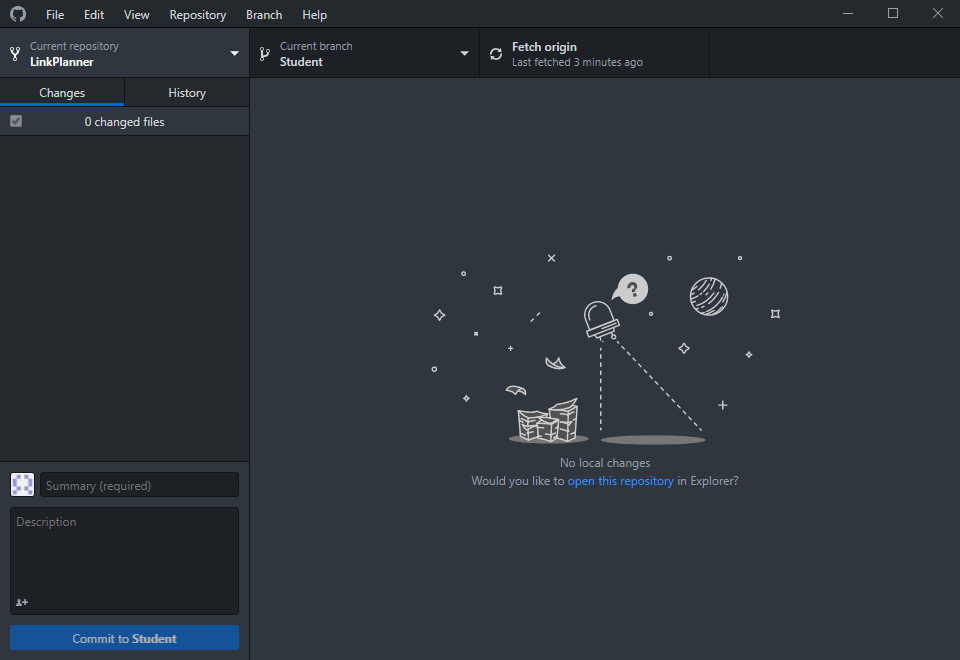
\includegraphics[width=.7\linewidth]{committing5}
\end{figure}
\end{frame}

\note[itemize]{
	\item This is what it looks like after pushing
}

\begin{frame}[t]{Committing, pushing and pulling}
\begin{figure}
\centering
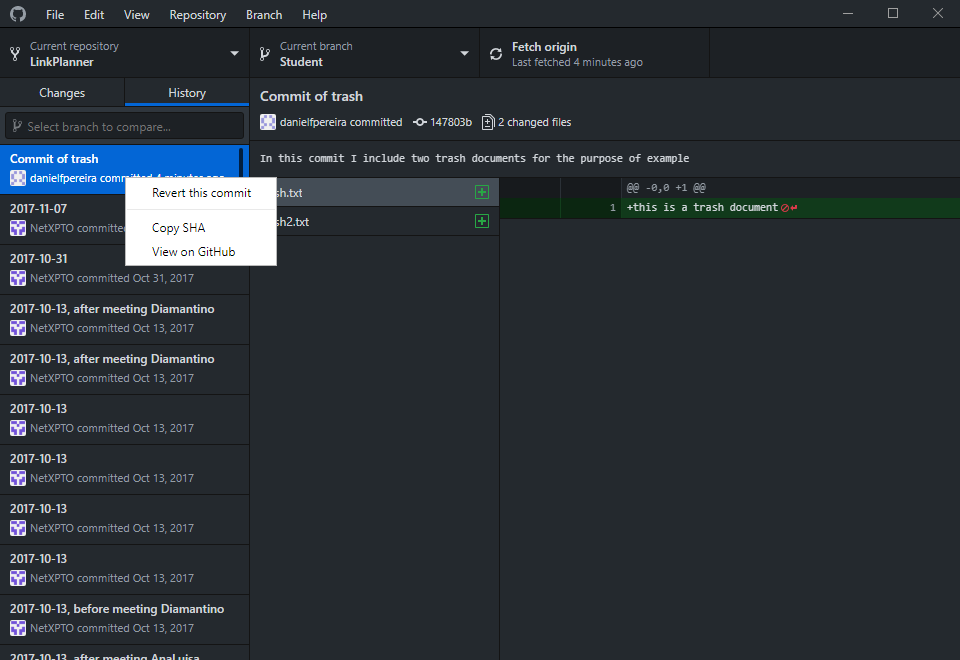
\includegraphics[width=.7\linewidth]{reverting1}
\end{figure}
\end{frame}

\note[itemize]{
	\item You revert a commit from the history tab
}

\subsection{Communicating between forks}
\begin{frame}[t]{Pull requests}
\begin{itemize}
\aitem The alterations you made and pushed to your account only live in your fork.
\aitem If you want to share them with someone else (for example the owner of the original repository) you need to open a pull request.
\end{itemize}
\end{frame}

\note[itemize]{
	\item After you committed and pushed your alterations, if you want to share your alterations, you need to request a pull from your account to theirs
}

\begin{frame}[t]{Pull requests}
\begin{figure}
\centering
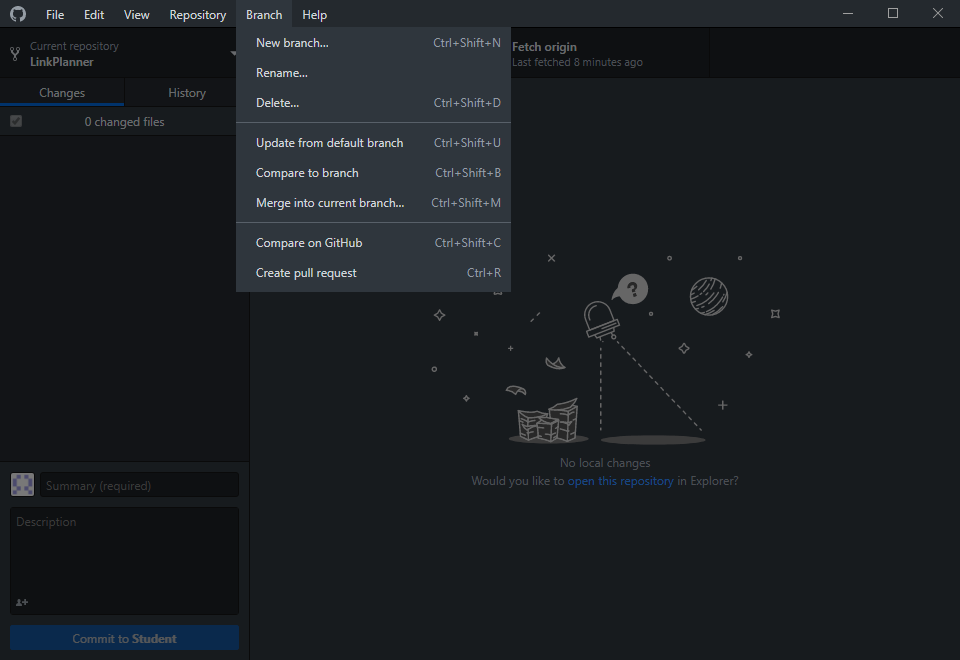
\includegraphics[width=.7\linewidth]{pullrequest1}
\end{figure}
\end{frame}

\note[itemize]{
	\item Go here on the desktop app, click Create pull request, this takes you to... NEXT SLIDE
}

\begin{frame}[t]{Pull requests}
\begin{figure}
\centering
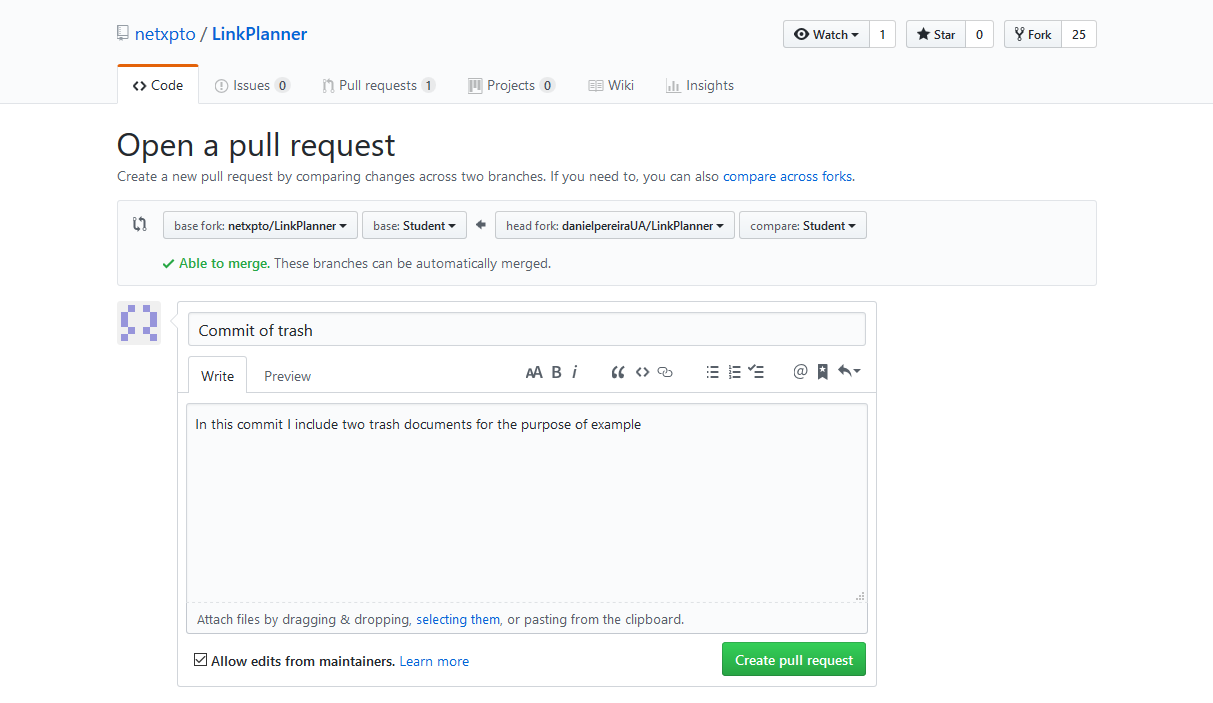
\includegraphics[width=.7\linewidth]{pullrequest2}
\end{figure}
\end{frame}

\note[itemize]{
	\item The website...
	\item Note the arrow, its direction
	\item Note the branches and forks on each side
	\item if you did everything right, it should say Able to merge, else it will tell you there are conflicts
	\item I'll explain what conflicts are after
}

\begin{frame}[t]{Pull requests}
\begin{itemize}
\aitem The alterations you made and pushed to your account only live in your fork.
\aitem If you want to share them with someone else (for example the owner of the original repository) you need to open a pull request.
\aitem The owner of the repository you are requesting the pull to needs to approve it before it actually happens.
\end{itemize}
\end{frame}

\note[itemize]{
	\item the owner of the repository being pulled to needs to authorize, he'll have to deal with the conflicts
}

\begin{frame}[t]{Pull requests}
\begin{itemize}
\aitem The alterations you made and pushed to your account only live in your fork.
\aitem If you want to share them with another fork of the same repository (for example original repository) you need to open a pull request.
\aitem The owner of the repository you are requesting the pull to needs to approve it before it actually happens.
\aitem Now say you want to update your fork from another fork of the same repository (for example, from the original repository).
\aitem You do the reverse of what you did previously.
\aitem Create a pull request from the fork you want to pull from into your fork.
\end{itemize}
\begin{figure}
\centering

\includegraphics[width=\linewidth]{pullrequest4}
\end{figure}
\end{frame}

\note[itemize]{
	\item now if you want to update your fork from an external fork, you do the same as before
	\item note the arrow
	\item Note the branches and forks on each side
}

\begin{frame}[t]{Pull requests}
\begin{figure}
\centering
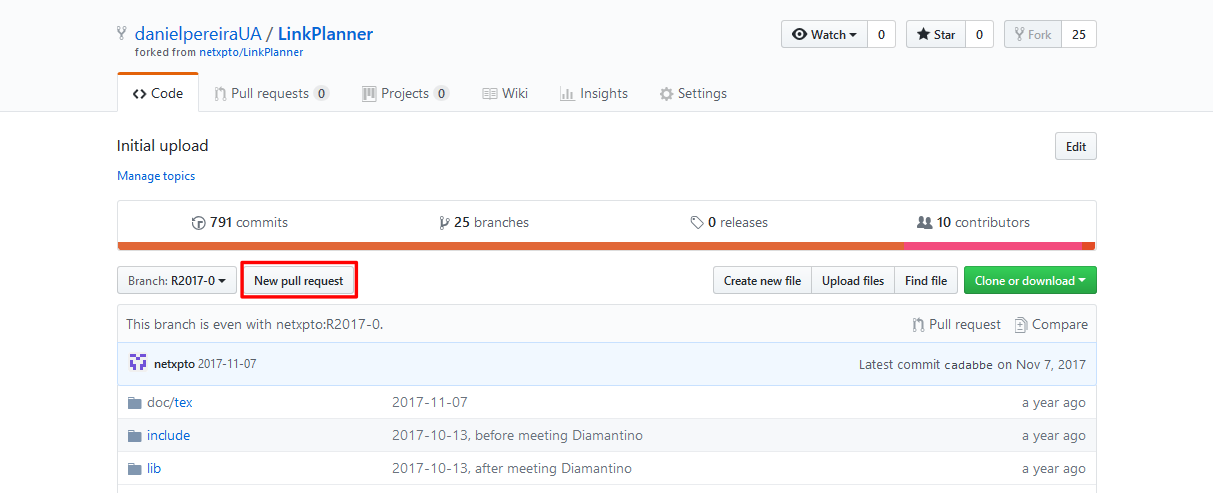
\includegraphics[width=\linewidth]{pullrequest3}
\end{figure}
\end{frame}

\note[itemize]{
	\item to get there, go to your repository's page and click here
}

\subsection{What if things go wrong?} % what to do if things go to shit?
\begin{frame}[t]{Conflicts}
\begin{itemize}
\aitem A conflict arises when:
\begin{itemize}
\bitem Change a file on PC A, push it to the cloud.
\bitem Change the same file on PC B before pulling the changes made on PC A.
\bitem When you then try to pull/push the changes made on PC A/B, you will have a conflict.
\end{itemize}
\aitem Git knows you made changes on both machines, it evens know what changes you made in which.
\aitem It needs you to tell it what changes to accept and what changes to discard.
\aitem This is called merging.
\end{itemize}
\end{frame}

\note[itemize]{
	\item what is a conflict?
	\item just follow the slide
}

\begin{frame}[t]{Conflicts}
\begin{figure}
\centering
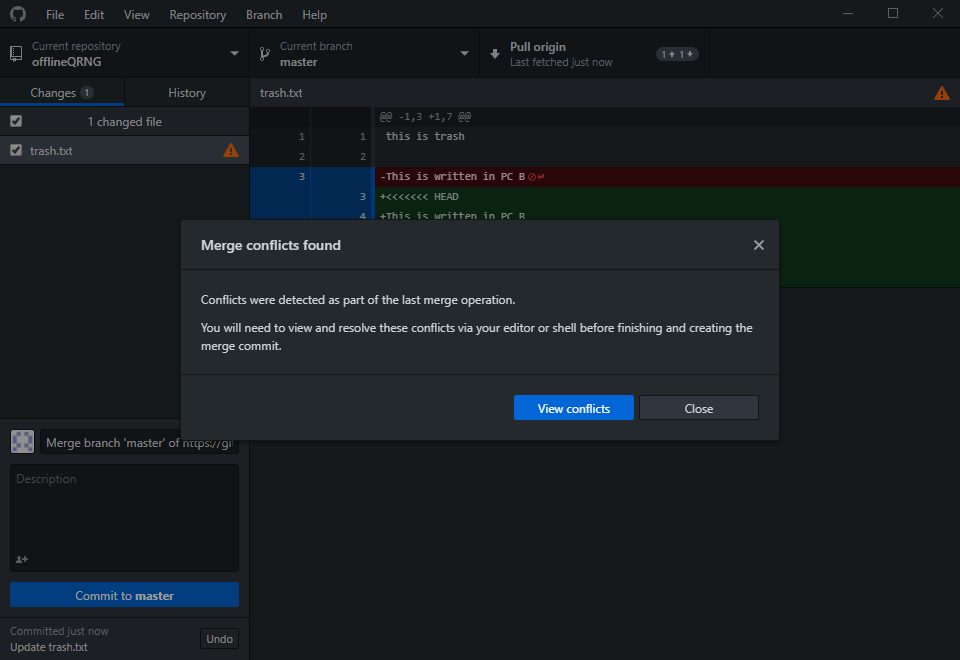
\includegraphics[width=.7\linewidth]{conflict1}
\end{figure}
\end{frame}

\note[itemize]{
	\item this is what the app will tell you
	\item note the danger logo
	\item there is a conflict on one file
}

\begin{frame}[t]{Conflicts}
\begin{figure}
\centering
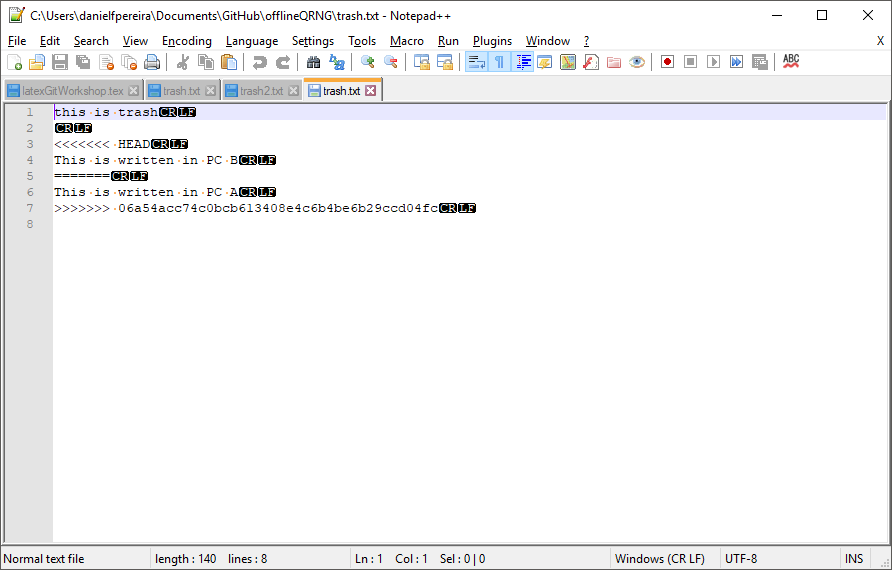
\includegraphics[width=.7\linewidth]{conflict2}
\end{figure}
\end{frame}

\note[itemize]{
	\item I am working on PC B
	\item Everything above the =============== line is what I have done in PC B
	\item Everything below the =============== line is what is in the cloud
	\item The text in the end identifies the commit in which what was in the cloud was added
}

\begin{frame}[t]{Conflicts}
\begin{figure}
\centering
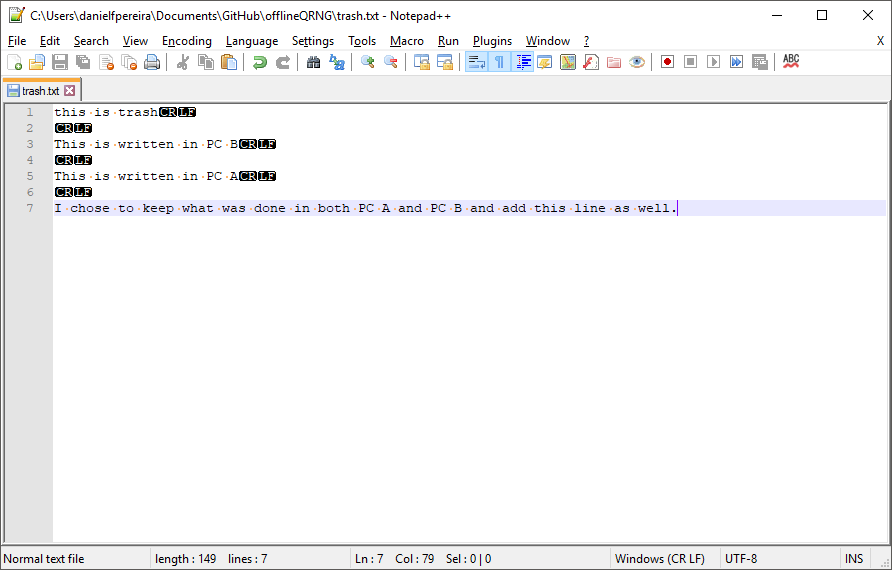
\includegraphics[width=.7\linewidth]{conflict3}
\end{figure}
\end{frame}

\note[itemize]{
	\item this is what a conflict solution may look like
	\item you may want to delete one of the versions
	\item you can write anything you want
}

\begin{frame}[t]{Conflicts}
\begin{figure}
\centering
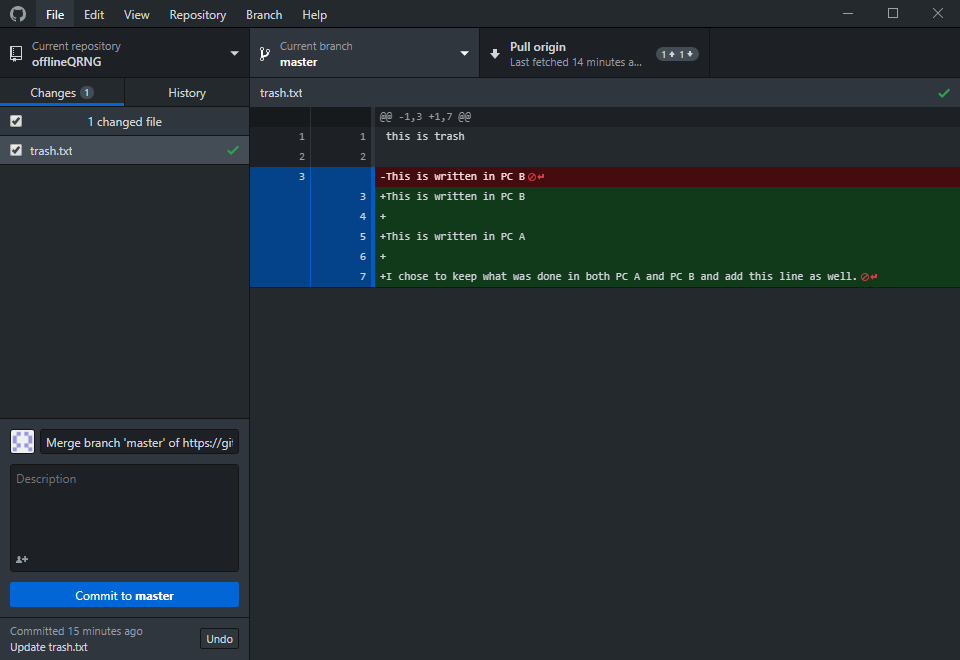
\includegraphics[width=.7\linewidth]{conflict4}
\end{figure}
\end{frame}

\note[itemize]{
	\item after the conflict has been solved
	\item note the danger logo is gone
	\item note the summary: it is automatically filled in by the app, you can change it if you want but I don't recommend it
}

\subsection{Summary}
\begin{frame}[t]{Topology of communications}
\begin{figure}
\centering
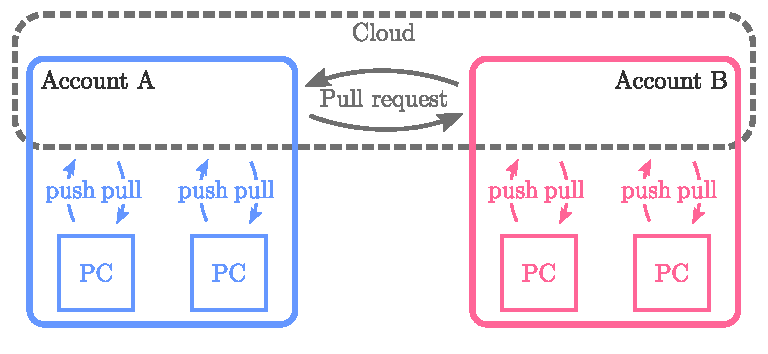
\includegraphics{gitTopology}
\end{figure}
\end{frame}

\note[itemize]{
	\item explain the whole figure
}

\subsection{This concludes the Git mini-workshop}
\note[itemize]{
	\item Any questions?
}

\section{The end!}

\end{document} 